\documentclass{beamer}

\usepackage{beamerthemesplit}
\usetheme{Singapore}

\input{../../include/preamble.inc} 
\input{../../include/definitions.inc} 
\input{../../include/author.inc} 

\title[]{Обтекание тел плоскими потенциальными течениями идеальной жидкости}

\begin{document}
	
\frame[plain]{\titlepage}


\frame[plain]{
	\frametitle{Аннотация}
	\parbox{\textwidth}{
		Обтекание абсолютно твердого тела. Задание граничных условий. Формулы Блазиуса -- Чаплыгина. Формулы Кутты -- Жуковского. 
	}
}

\frame{
	\frametitle{ Задача обтекания абсолютно твердого тела }
	
	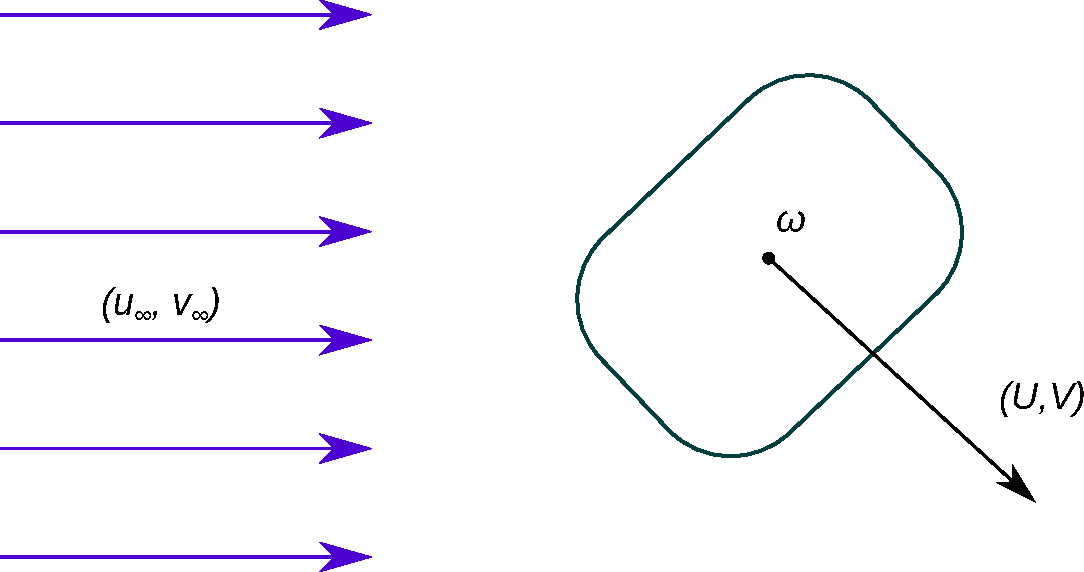
\includegraphics[width=\linewidth]{../img/flow_body.pdf}
}


\frame{
	\frametitle{ Математическая постановка задачи обтекания тела потенциальным потоком идеальной жидкости}

	\begin{exampleblock}{}
	\parbox{\textwidth}{
		Требуется найти \alert{аналитический комплексный потенциал}
		\[
			w(z) = \varphi(x,y) + i \psi(x,y),\quad
			z = x + i y,
		\]
		определенный в рассматриваемой бесконечной области, связанный соответствующими условиями на бесконечности и границе с телом и такой, что 
		\[
			\Delta \psi(x,y) = 0.
		\]
	}
	\end{exampleblock}

	\begin{exampleblock}{Замечание}
		\smallskip
		\parbox{\textwidth}{
			Так как потенциал $\varphi$ связан с функцией тока $\psi$ соотношениями Коши -- Римана, то функция тока находится автоматически. Можно, наоборот, искать потенциал $\varphi$, а $\psi$ выражать через соотношения Коши -- Римана.
		}
	\end{exampleblock}
	
}


\frame{
	\frametitle{ Плоское покоящееся течение на бесконечности }
	
	\begin{exampleblock}{Условия на бесконечности}
		\smallskip
		\parbox{\textwidth}{
		\[
			\pd{\psi}{x} = 0,\quad
			\pd{\psi}{y} = 0
		\]
		для бесконечно удаленных точек пространства, т.к. скорость на бесконечности равна $0$.
		}
	\end{exampleblock}
}

\frame{
	\frametitle{ Условие <<непротекания>> на границе с телом }
	
	\begin{columns}
		\begin{column}{0.4\textwidth}
			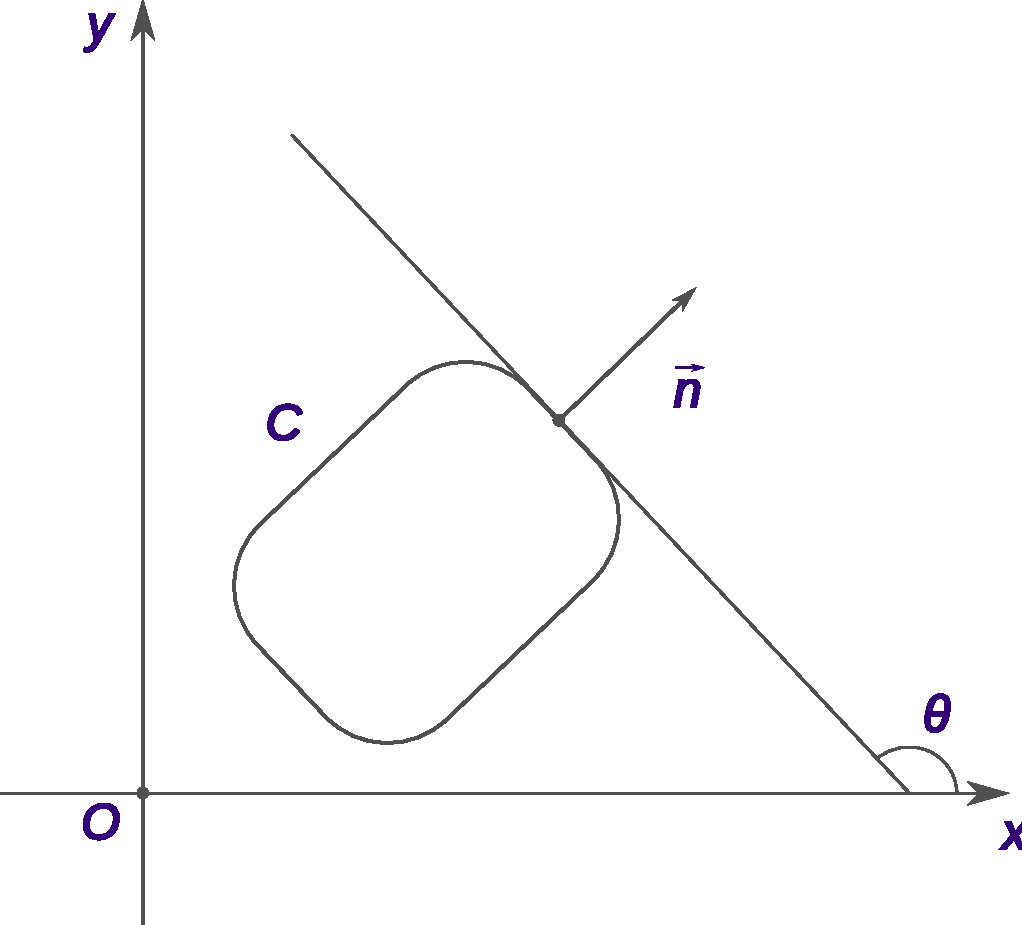
\includegraphics[width=\linewidth]{../img/vn.pdf}
		\end{column}
		\begin{column}{0.6\textwidth}
			\begin{exampleblock}{Условие на границе с телом}
				\parbox{\textwidth}{
					Нормальная составляющая (относительно границы тела) скорость течения должна совпадать с нормальной составляющей скорости тела.
				}
			\end{exampleblock}
		\end{column}
	\end{columns}

	\parbox{\textwidth}{
		\[
		v_n = v_x \cos(\vec{n},x) +v_y \cos (\vec{n},y) = v_x \sin\theta - v_y \cos\theta=
		\]
		\[
		=
		v_x\od{y}{s}-v_y\od{x}{s} = \pd{\psi}{y}\od{y}{s}+\pd{\psi}{x}\od{x}{s} = \pd{\psi}{s},
		\]
		где $x(s)$, $y(s)$ -- параметризованная граница тела в окрестности рассматриваемой точки.
	}

}

\frame{
	\frametitle{ Условие для движения абсолютно твердого тела}
	
	\parbox{\textwidth}{
	Пусть тело совершает поступательное движение со скоростью $(U,V)$ и вращательное движение с угловой скоростью $\omega$, тогда скорости точек тела будут иметь вид:
	\[
	u_x = U - \omega y,\quad
	u_y = V+\omega x,
	\]
	где $(x,y)$ -- координаты точек тела во вращающейся системе координат, жестко связанной с телом.
	}	\pause

	
	\begin{exampleblock}{Условие на границе с телом}
		\parbox{\textwidth}{
			\[
		\pd{\psi}{s} = 
		u_x \cos (\vec{n},x) + u_y \cos (\vec{n},y)	=
		u_x \od{y}{s} - u_y \od{x}{s} =
		\]
		\[
		=
		(U - \omega y)\od{y}{s} - (V+\omega x) \od{x}{s}
		\]	
		
		Отсюда,
		\[
		\psi = U y - V x -\frac{1}{2}\omega(x^2+y^2) + c.
		\]
		}
	\end{exampleblock}
	

	
}

\frame{
	\frametitle{ Частный случай набегающего потока на покоящееся тело }
	
	\begin{exampleblock}{Условие на границе тела}
		\parbox{\textwidth}{
			В случае покоящегося тела $U=V=0$, $\omega=0$ условие на границе тела будет:
			\[
				\psi(x,y) = const.
			\]
			
		}
	\end{exampleblock}

	\begin{exampleblock}{Условие на бесконечности}
		\smallskip
		\parbox{\textwidth}{
			В случае набегающего потока с параметрами на бесконечности 
			\[
			v_x=v_\infty,\quad 
			v_y = 0,
			\]
			условие для бесконечно удаленных точек будет:
			\[
			\psi(x,y) = v_\infty y + const.
			\]
		}
	\end{exampleblock}
	
}

\frame{
	\frametitle{ Задача обтекание тела }
	
		\parbox{\textwidth}{
			Таким образом, задача обтекания тела плоским потенциальным потоком идеальной жидкости сводится к решению \alert{задачи Ди\-рих\-ле} для функции тока $\psi$: 
			\begin{enum}
				\item
			внутри исследуемой области решается уравнение Лапласа:
			\[
			\Delta \psi = 0;
			\]
			\item
			а на бесконечности и границе обтекаемого тела заданы значения функции $\psi$ в зависимости от условий обтекания.
			\end{enum}
			
			
		}
	
}

\frame{
	\frametitle{ Сила  при безотрывном обтекании }
	
	\begin{exampleblock}{Определение}
		\parbox{\textwidth}{
			По аналогии с комплексными скоростью и потенциалом определим комплексную силу $R$, действующую на контур $C$ в области течения по формуле
			\[
			R = X + i Y,
			\]
			где $X$, $Y$ -- вещественные проекции силы на оси координат.
			
		}
	\end{exampleblock}	
}

\frame{
	\frametitle{ Формула для силы через давление при безотрывном обтекании}
	
	\centering
	\begin{columns}
		\begin{column}{0.5\textwidth}
			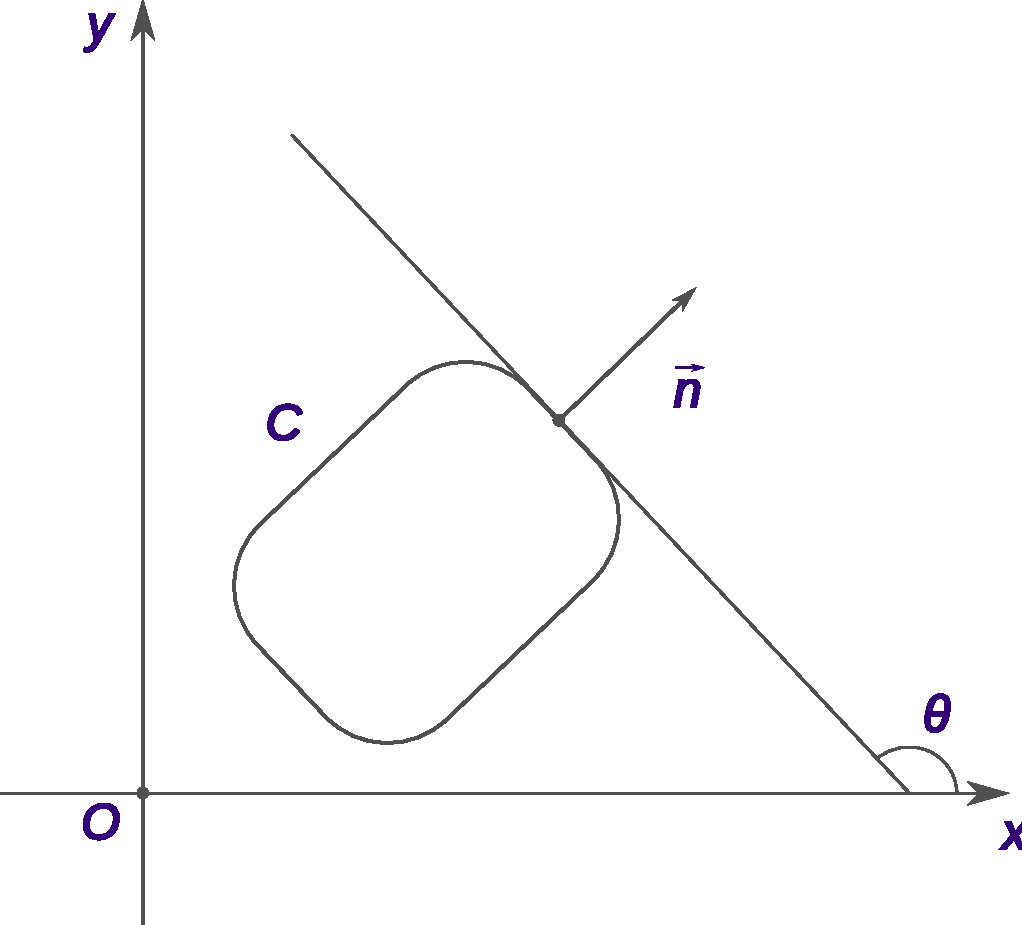
\includegraphics[width=\linewidth]{../img/vn.pdf}
		\end{column}
		\begin{column}{0.5\textwidth}
			\begin{exampleblock}{}
				\parbox{\textwidth}{
					Комплексно-сопряженная сила $R^*$ вдоль контура тела $C$ при безотрывном обтекании:
					\[
					R^* = X - i Y = 
					\]
					\[
					=
					-\oint\limits_C p (\cos(\vec{n},x) - i \cos(\vec{n},y)) ds = 
					\]
					\[
					=
					-\oint\limits_C p (\sin\theta + i \cos\theta) ds = 
					\]
					\[
					=
					-i \oint\limits_C p e^{-\theta i} ds.
					\]
					
					
				}
			\end{exampleblock}
		\end{column}
	\end{columns}
		

}

\frame{
	\frametitle{ Предварительные выкладки }
	
	\begin{exampleblock}{Выражение для комплексного дифференциала}
		\parbox{\textwidth}{
			\[
			dz = dx + i dy = ds(\cos\theta + i \sin\theta) = e^{i\theta}ds,
			\]
			\[
			dz^* = dx - i dy = ds(\cos\theta - i \sin\theta) = e^{-i\theta}ds.
			\]
			Отсюда
			\[
			dz^* = e^{-2\theta i} dz.
			\]
			
		}
	\end{exampleblock}\pause

	\begin{exampleblock}{Интеграл Бернулли}
		\parbox{\textwidth}{
			Связь давления и скорости через интеграл Бернулли
			\[
				p = c - \frac{1}{2}\rho v^2
			\]
			справедлива вдоль контура тела при безотрывном обтекании, т.к. он является линией тока. При потенциальном течении эта связь справедлива во всей области течения.
			
		}
	\end{exampleblock}

	
}


\frame{
	\frametitle{ Сила }
	
	
	\begin{exampleblock}{}
		\parbox{\textwidth}{
		\[
			R^* = -i c \oint\limits_{C}d z^* + \frac{i \rho}{2} \oint\limits_C v^2 dz^*=
			\frac{i \rho}{2} \oint\limits_C v^2 dz^*=
			\frac{i \rho}{2} \oint\limits_C (v e^{-i \theta})^2 dz
		\]\pause
		
		Используя, что
		\[
		v e^{-i \theta} = v \cos\theta -i v \sin\theta = v_x-i v_y = v^*,
		\]
		получим:
		\[
		R^* = X - i Y = \frac{i\rho}{2} \oint\limits_C (v^*)^2 dz.
%		 = \frac{i\rho}{2} \oint\limits_C \left(\od{w}{z} \right)^2 dz
		\]
		
		}
	\end{exampleblock}
}

\frame{
	\frametitle{ Момент главных сил }
	\parbox{\textwidth}{
	\[
	L = -\oint\limits_C p (x \cos(\vec{n},y)-y\cos(\vec{n},x)) ds =
	-\oint\limits_C p (x \cos\theta + y\sin\theta) ds =
	\]
	\[
	=
	-\oint\limits_C p (x dx + y dy) =
		-\oint\limits_C \left(c + \frac{\rho v^2}{2}\right) (x dx + y dy) =
	\]
	\[
	=
	-\oint\limits_C c\, d(x^2+y^2) - \frac{\rho}{2}\oint\limits_C v^2 (x dx + y dy)=
%	\]
%	\[
%	= 
	\Re \left( 
	-\frac{\rho}{2}\oint\limits_C v^2zdz^*
	\right)=
	\]
	\[
	=
	\Re \left( 
	-\frac{\rho}{2}\oint\limits_C (v^*)^2zdz,
	\right),
	\]
	т.к. $v^2 dz^* = (v^*)^2 dz$.
	}
	
}

\frame{
	\frametitle{ Формулы Блазиуса -- Чаплыгина для потенциального течения }
	
	\begin{exampleblock}{ }
		\parbox{\textwidth}{
			Если течение потенциально, тогда существует комплексный потенциал:
			\[
			w(z)= \varphi(z) + i \psi(z) \quad\text{и}\quad
			\od{w}{z} = v^*.
			\]
		}
	\end{exampleblock}

	\begin{exampleblock}{ Формулы Блазиуса -- Чаплыгина }
		\parbox{\textwidth}{
		\[
		R^* = X - i Y = \frac{i\rho}{2} \oint\limits_C \left(\od{w}{z} \right)^2 dz,
		\]	
		\[
		L = \Re \left[
		-\frac{\rho}{2}\oint\limits_C \left(\od{w}{z} \right)^2 zdz
		\right].
		\]
		}
	\end{exampleblock}
}

\frame{
	\frametitle{ Формула Кутты -- Жуковского }

\begin{exampleblock}{Предположения }
	\parbox{\textwidth}{
		Поток потенциален вне тела, которое можно заменить на конечное число источников, вихрей и диполей, лежащих внутри границы тела -- контура $C$.
	}
\end{exampleblock}


\begin{exampleblock}{Формула для силы и реакции}
	\parbox{\textwidth}{
		\[
		R^* =  X - iY = i\rho\Gamma v_\infty^*,		
		\]
		\[
		L = \Re \left[
		-\rho v_\infty^*\sum\limits_{k=1}^m\Gamma_kb_k-i\rho M v_\infty^*
		\right],
		\]
		где
		$\Gamma_i$ -- циркуляции вихрей, находящихся в точках $b_i$ $(i=1,\ldots,m)$; $M$ -- суммарный момент источников и диполей; $\Gamma$ -- суммарная циркуляция вихрей, находящихся внутри тела.
	}
\end{exampleblock}

}


\frame{
	\frametitle{Метод конформных отображений}
	
	\begin{exampleblock}{Основная идея}
		\parbox{\textwidth}{
			Использование \textit{метода конформных отображений} и \textit{теоремы Римана о конформном отображении односвязных областей.}
		}
	\end{exampleblock}


	\begin{exampleblock}{ Дано }
		\begin{enumerate}
			\item  комформное отображение $z=f(\zeta)$;
			\item  потенциал течения на вспомогательной плоскости $\psi(\zeta)$.
		\end{enumerate}
	\end{exampleblock}

	\begin{exampleblock}{Решение}
		\parbox{\textwidth}{
				\[
			\left\{
			\begin{array}{l}
				\chi = \chi(f(\zeta)) = \psi(\zeta),\\
				z = f(\zeta).
			\end{array}
			\right.
			\]
						\[
			v^* = \od{\chi}{z} = \od{\psi}{\zeta}  \od{\zeta}{z},
			\]
			где $\chi(z)$ --- потенциал течения в физической плоскости.
		}
	\end{exampleblock}
	 
}


\frame{
	\frametitle{Задача обтекания кругового цилиндра}
	
	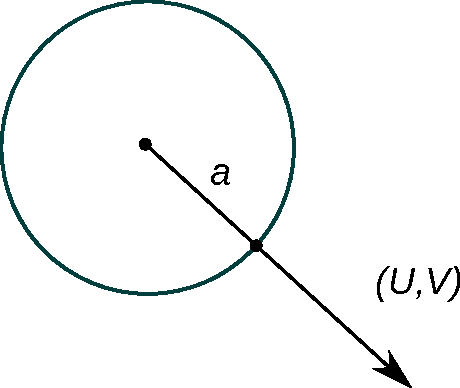
\includegraphics[width=0.5\linewidth]{../img/flow_cylinder.pdf}
	
	\begin{exampleblock}{}
		\parbox{\textwidth}{
			Найти комплексный потенциал обтекания кругового цилиндра радиуса $a$, движущегося в бесконечной покоящейся жидкости со скоростью $(U,V)$.
		}
	\end{exampleblock}	
		
}

\frame{
	\frametitle{ Задача обтекания кругового цилиндра }
	
	
	\begin{exampleblock}{Постановка задачи}
		\parbox{\textwidth}{
			\only<1>{
				В системе координат цилиндра найти потенциал % $w(z)$
				\[
				w(z) = \varphi(z) + i \psi(z)
				\]
				такой, что его мнимая часть на окружности $|z| = a$ удовлетворяет условию
				\[
				\psi(x+iy) = U y - V x + \mathrm{const}.
				\]
			}
		
			\only<2>{
				Решение ищется в виде ряда:
				\[
				\od{w}{z} = v^*(z) = c_0 + \frac{c}{z} + \frac{c_1}{z^2} + \frac{c_2}{z^3} + \ldots,
				\]
				т.к. $v^*(z)$ -- однозначна, определена вне $|z|>a$, ограничена и на бесконечности стремится к $0$.
				
				Сразу следует, что 
				\[
				c_0 = 0
				\]
				и
				\[
				w(z) = c \ln(z) + \sum_{n=1}^{\infty}\frac{c_n}{z^n}.
				\]
			}
			\only<3>{
				Для обеспечения выполнения граничных условий необходимо
				\[
				\left. \pd{\varphi}{r} \right|_{r=a} = U \cos \theta + V \sin \theta.
				\]
				
				При $c = A + iB$, $c_n = A_n + i B_n$, $z=r e^{i\theta}$
				\[
					w(z) = \varphi+i \psi = (A + iB) (\ln r + i \theta) +
					(A_1 + i B_1) \frac{1}{r} (\cos \theta - i \sin \theta) +
				\]
				\[
					+\sum_{n=2}^\infty (A_n + i B_n) \frac{1}{r^n} (\cos n\theta - i \sin n\theta).
				\]
			}
		
			\only<4>{
				Таким образом,
				\[
					\varphi(r) =  Re(w(z)) = A \ln r - B\theta + (A_1 \cos\theta + B_1 \sin\theta)\frac{1}{r} +
				\]
				\[
				+ \sum_{n=2}^\infty \frac{1}{r^n} (A_n \cos n\theta + B_n \sin n\theta).
				\]
				\[
				\pd{\varphi}{r} = \frac{A}{r} - (A_1 \cos\theta + B_1 \sin\theta)\frac{1}{r^2} -
				\sum_{n=2}^\infty \frac{n}{r^{n+1}} (A_n \cos n\theta + B_n \sin n\theta).
				\]
			
			}
			\only<5>{
				Полагая $r=a$,
				\[
				\left.\pd{\varphi}{r}\right|_{r=a} = \frac{A}{a} - (A_1 \cos\theta + B_1 \sin\theta)\frac{1}{a^2} -
				\sum_{n=2}^\infty \frac{n}{a^{n+1}} (A_n \cos n\theta + B_n \sin n\theta) = 
				\]
				\[
					 = U \cos\theta + V \sin\theta.
				\]
				
				Следовательно,
				\[
				A = 0,\quad
				A_1 = -U a^2,\quad
				B_1 = -V a^2,\quad
				A_n = B_n = 0.
				\]
				Коэффициент  $B$ остался не определён. Положим $B = -\displaystyle\frac{\Gamma}{2 \pi}$, тогда
				\[
				w(z) = \frac{\Gamma}{2 \pi i} \ln z - \frac{U a^2 + i V a^2}{z}.
				\]
			}
		
			
		}
	\end{exampleblock}



}



\frame{
	\frametitle{ Задача обтекания кругового цилиндра }
	
	\begin{exampleblock}{Решение}
		\parbox{\textwidth}{
			\begin{eqnarray*}
				w(z)  & = & \frac{\Gamma}{2\pi i }\ln z - (U + i V)\frac{a^2}{z}, \\
				\varphi(z) & = & \frac{\Gamma}{2\pi \theta } - (U \cos \theta + V \sin \theta)\frac{a^2}{r}, \\
				\psi(z) & = & -\frac{\Gamma}{2\pi } \ln r + (U \sin \theta - V \cos \theta)\frac{a^2}{r}, \\
			\end{eqnarray*}
			где  $z=r e^{i \theta}$.
		}
	\end{exampleblock}
	
}


\frame{
	\frametitle{Задача обтекания кругового цилиндра жидкостью, {\em движущейся на бесконечности} }
	
	\begin{exampleblock}{Решение}
		\smallskip
		\parbox{\textwidth}{
			Потенциал для задачи обтекания круга поступательным потоком, имеющим на бесконечности скорость $v_\infty = v_{\infty,x} + i v_{\infty,y}$, имеет вид:
			\[
			w(z) = v_\infty^*z + (v_\infty -  U - i V)\frac{a^2}{z} + \frac{\Gamma}{2\pi i }\ln z.
			\]
			
			Интересный случай --- обтекание неподвижного цилиндра $U=V=0$. 
		}
	\end{exampleblock}
}



\frame{
	\frametitle{ Литература }
	\begin{literature}
		\item
		{\em Валландер С.\,В.}
		Лекции по гидрофэромеханике. Учеб. пособие. Л. Изд-во Ленингр. ун-та, 1978.
		
		\item 
		{\em Кочин~Н.~Е., Кибель~И.~А., Розе~Н.~В.} Теоретическая гидромеханика. М.: Гос. издат. физ.-мат. лит., 1963.
		
	\end{literature}
}

\end{document}